\documentclass[main.tex]{subfiles}
% 标架与参考系
\begin{document}
\subsection{引子}
经典力学中,物理事件的发生是不依赖于人的观察与否或观察方式的客观事实。我们希望,同一件物理事件,经不同的观察者观察后作出的报告,能通过一套互译系统而统一成一个结论;从而,通过对实验观测的总结归纳,可以达成一个不依赖具体观察者的情境和观察方式的、关于大自然规律性的共识。

\begin{figure}[h]
    \centering
    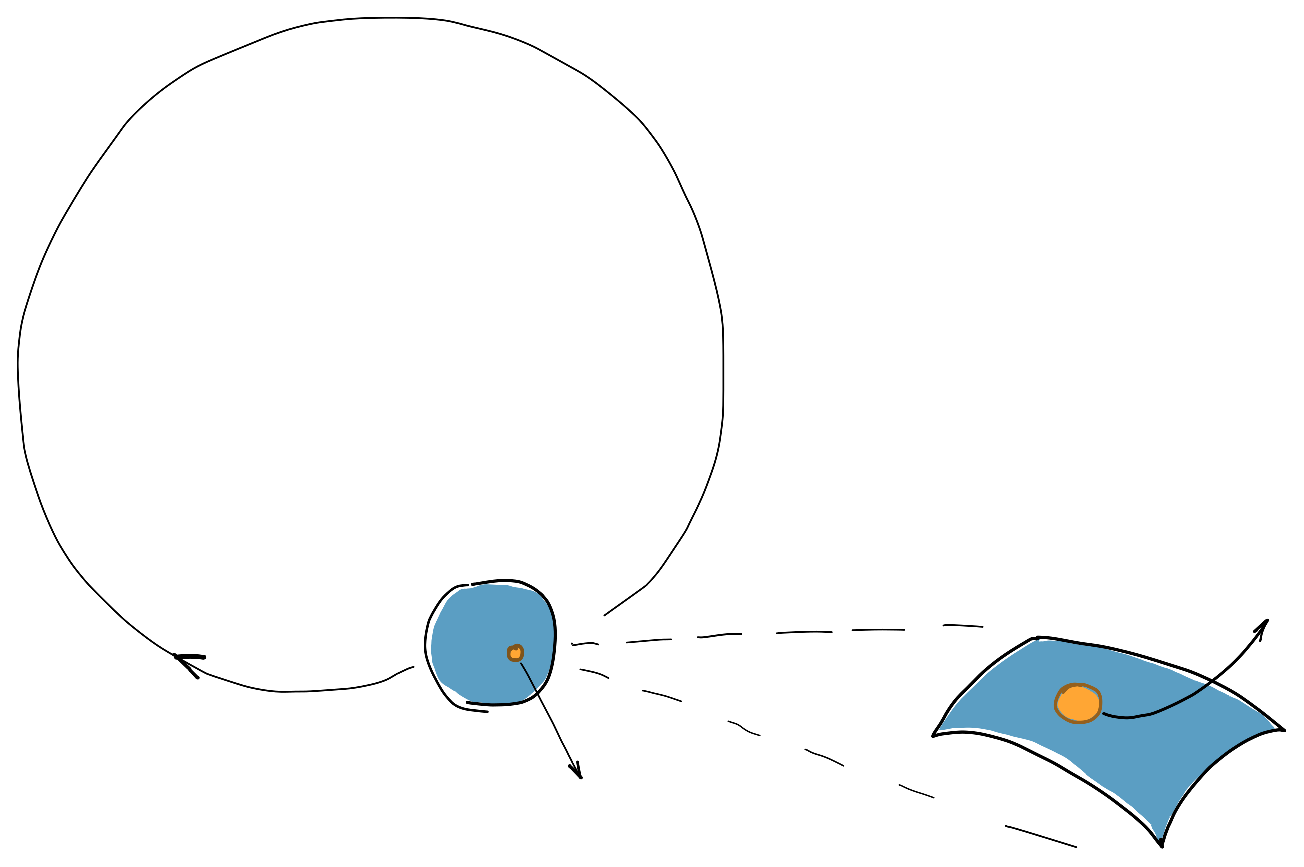
\includegraphics[width=0.5\textwidth]{images/III.1.1.eps}
    \caption{非惯性系下的运动规律。}
    \label{fig:III.1.1}
\end{figure}

\begin{example}[非惯性系]
在一个相对我们作低速圆周运动的球上站着的人(他看不到我们,但能与我们通讯交流),通过抓稳该球保持与球相对静止。他以球作参照物,研究球上的物体的运动,会得出:保持物体的静止需要一个方向恒定的力,因为球上的物体都需要绑在球上才能保持相对于球静止,他通过弹簧秤可以测量出这一力的大小。如果把某物体松绑,使其不受任何力,物体会开始作一个曲线运动。我们则能不通过测量力就看到球和球上的物体的圆周运动,在我们眼中它们的运动状态是一直在改变中的,而不是静止的;给物体松绑后,物体以松绑时的速度作为初速度作均速直线运动(如图\ref{fig:III.1.1}所示)。如果球做圆周运动的角速度发生变化,我们仍然能不通过力的测量而看到这一点,但球上的人只会发现,保持球上物体静止所需的力的大小在莫名其妙地变化。如果他在球上设置一个单摆,他将发现单摆的摆动方向在随时间变化,而我们认为没有变化。总而言之,我们认为牛顿力学定律符合实际,但他将不会同意。但他和我们都坚信,大家所观察的现象是同一个物理现象,受同一套自然定律统治。摆在他和我们面前的任务只是如何统一地描述好这一自然定律。
\end{example}

\subsection{时间、空间、标架、参考系}
在经典力学中,一个物理事件的发生,同时具有“发生的位置”和“发生的时刻”这两个属性。一名观察者使用时钟测量两个物理事件发生的时间间隔。这名观察者还使用直尺来测量两个物理事件发生位置之间的距离,且这种测量总是只能针对同时刻发生的两个事件。以下的数学构建,都是为了模拟上述的直观体验。

引入事件世界$\mathcal{W}$。$\mathcal{W}$是一个非空集,其元素$w\in\mathcal{W}$称为一个事件。我们给予$\mathcal{W}$一个函数$\tau:\mathcal{W}^2\rightarrow\mathbb{R}$,满足:
\begin{itemize}
    \item $\forall a,b\in\mathcal{W}:\tau\left(a,b\right)=-\tau\left(b,a\right)$
    \item $\forall a,b,c\in\mathcal{W}:\tau\left(a,b\right)+\tau\left(b,c\right)=\tau\left(a,c\right)$
    \item $\forall a\in\mathcal{W},t\in\mathbb{R},\exists b\in\mathcal{W}:\tau\left(a,b\right)=t$
\end{itemize}
我们称$\tau$为(两事件的)时间间隔或时长。我们还能称
\begin{itemize}
    \item 事件$a$早于事件$b$当且仅当$\tau\left(a,b\right)>0$
    \item 事件$a$晚于事件$b$当且仅当$\tau\left(a,b\right)<0$
    \item 事件$a$与$b$同时当且仅当$\tau\left(a,b\right)=0$
\end{itemize}
上面的第三条给出了两事件的同时性。易验同时性是一个等价关系,即$S=\left\{\left(a,b\right)|\tau\left(a,b\right)=0\right\}$满足自反性、传递性、对称性。这一等价关系将事件世界$\mathcal{W}$划分为等价类,即:
\[\mathcal{W}=\bigcup_{a\in\mathcal{T}}I_a,I_a=\left\{x\in\mathcal{W}|\tau\left(a,x\right)=0\right\}\]
其中等价类$I_a$称为时刻,是所有与事件$a$同时的事件的子集,而$a$在此变成了时记得的标记,集合$\mathcal{T}$就是所有(不同)时刻的集合。

我们还给予事件世界$\mathcal{W}$以一个度量$d:I_a\times I_a\rightarrow\mathbb{R},a\in\mathcal{T}$,称两事件间的“距离”,它还要满足:
\begin{itemize}
    \item $d$是$I_a$上的一个欧几里德度量,故$I_a$是一个欧几里德空间,带有一个平移空间$\mathcal{V}_a$。
    \item $\forall a\in\mathcal{T}:\mathrm{dim}\mathcal{V}_a=3$
\end{itemize}
注意到,这一度量只能作用在同时发生的两个事件上的。

结合度量$\tau$的定义,$\left(\mathcal{T},\left|\tau\right|\right)$形成一个度量空间。在此度量空间上的等距变换拥有之前介绍过的一切性质。值得注意的是,由$\tau$的定义,可知$\mathcal{T}$的平移空间是一维的、完备的。我们可直接使用实数集$\mathbb{R}$作为其平移空间。选定某时刻$t_0\in\mathcal{T}$作为原点,$\mathbb{R}$的正或负作为时间流逝的方向以及单位时长(相当于在作为向量空间的$\mathbb{R}$中选择了一个规范正交基),则对任一$\mathcal{T}$上的等距变换$i:\mathcal{T}\rightarrow\mathcal{T}$有$i\left(t\right)=i\left(t_0\right)+ Q\left(t-t_0\right)$。其中$Q=\pm 1$时间正方向的选择。由于我们很少遇到两个观察者记录时间的方式是反号的情况,因此常常只讨论(默认)$Q=1$。

一名观察者对任一事件$w\in\mathcal{W}$的观测,就是说出这一事件发生的时刻和空间位置。设以映射$\phi:\mathcal{W}\rightarrow\mathcal{E}\times\mathcal{T}$描述这一观测,则其中的欧几里德空间$\mathcal{E}$是与$\mathcal{T}$中的时刻相对应的那个同时等价类。我们还规定映射$\phi$是可逆的。具体地,一名观察者自行确定一个时间原点,使得$\mathcal{T}$与其平移空间$\mathbb{R}$构成双射,任一时刻$t\in\mathcal{T}$唯一对应一个实数。同时,该名观察者也自行确定了一个空间原点和直角坐标系,使得点集$\mathcal{E}$与其平移空间$\mathcal{V}$的向量构成双射, 且$\mathcal{V}$选定了一组规范正交基,使得任一点$X\in\mathcal{E}$唯一对应一个有序实数三原组。

我们罗列一下,上述观测过程中的要素,哪些是观察者的主观选择,哪些是客观的(即不依赖观察者)。客观的有:
\begin{itemize}
    \item 事件世界$\mathcal{W}$的所有事件
    \item 时间$\mathcal{T}$中的所有时刻和时延函数$\tau$
    \item 空间点集$\mathcal{E}$中的所有点其量度$d$以及平移空间$\mathcal{V}$
\end{itemize}
由观察者选择的有:
\begin{itemize}
    \item 空间原点和规范正交基(坐标系)
    \item 时间原点、单位时长和时间流逝的正方向
\end{itemize}
映射$\phi$作为对某观察者的观测行为的描述,包括且仅包括上述观察者的主观选择的对应性。此外,$\phi$还包括观察者进一步选择非规范正交基(例如某曲线坐标系)的可能。所以,具体而言,映射$\phi$是将一个物理事件对应到一个有序实数四元组,$\phi:\mathcal{W}\rightarrow\mathbb{R}^4$。但本讲义按照大多数资料中的惯例,仍把$\phi$简记为$\phi:\mathcal{W}\rightarrow\mathcal{E}\times\mathcal{T}$。

我们称$\phi$是一个标架。它代表了一个观察者如何将一个或若干个客观的物理事件用有序实数四元组表出的具体方式。一般地不同观察者在这一行为当中的区别就是标架的区别,故标架就是观察者、观察者就是标架。我们还称标架$\phi$的陪域为一个参考系。由上述的说明,这个陪域实际上是多元组$\left(O,\left\{\mathbf{\hat{e}}_i\right\}\right)\times\left(t_0,\text{单位时长},\text{正方向}\right)$,但本讲义按照大多数资料中的惯例,仍称$\mathcal{E}\times\mathcal{T}$为参考系。两个参考系不同当且仅当参考系的多元组$\left(O,\left\{\mathbf{\hat{e}}_i\right\}\right)\times\left(t_0,\text{单位时长},\text{正方向}\right)$有所不同,而两个标架的不同,除了参考系的不同外,还可能是选用的非规范正交基不同(如选用了某曲线坐标系)。

\subsection{标架变换}
两个标架$\phi:\mathcal{W}\rightarrow\mathcal{E}\times\mathcal{T},\phi^*:\mathcal{W}\rightarrow\mathcal{E}^*\times\mathcal{T}^*$,它是两个观察者对同一组物理事件的观测。我们称$\left(\phi,\phi*\right)$称为一个标架变换当且仅当这两个标架的时间单位和方向相同且标架间的变换是等距变换。

具体地,任一事件$w\in\mathcal{W}$经标架$\phi$映射为$\left(\mathbf{x},t\right),\mathbf{x}\in\mathbb{R}^3,t\in\mathbb{R}$,经标架$\phi^*$映射为$\left(\mathbf{x}^*,t^*\right),\mathbf{x}^*\in\mathbb{R}^3,t^*\in\mathbb{R}$。由于标架是可逆的,故有$\left(\mathbf{x}^*,t^*\right)=\phi^*\circ\phi^{-1}\left(\mathbf{x},t\right)$。若$w$的时刻是$a\in\mathcal{T}$,标架$\phi$选择的时间原点是$t_0$,标架$\phi^*$选择的时间原点是$t_0^*$,则时间的度量空间上的一个等距变换$g:\mathcal{T}\rightarrow\mathcal{T}$可表示为
\[t^*=g\left(t\right)=t_0^*+\tau\left(t-t_0\right),t_0^*=g\left(t_0\right)\]
$\mathcal{E}$和$\mathcal{E}^*$都是时刻$a$对应的同时等价类。若标架$\phi$和$\phi^*$选择的空间原点分别是$\mathbf{x}_0,\mathbf{x}_0^*$,则由$\mathcal{E}$到$\mathcal{E}^*$的一个等距变换$i_a:\mathcal{E}\rightarrow\mathcal{E}^*$可表示为
\[\mathbf{x}^*=i_a\left(\mathbf{x}\right)=i_a\left(\mathbf{x}_0\right)+\mathbf{Q}_a\left(\mathbf{x}-\mathbf{x}_0\right),\mathbf{x}_0^*=i_a\left(\mathbf{x}_0\right)\]
所以,由$\phi$到$\phi^*$的标架变换包含一个时间的等距变换$g$和一个空间的等距变换$i_a$,其中$a$是事件的时刻。

一名观察者无法直接认识抽象的事件本身,他能且只能对事件进行观测,即某标架$\phi$映射后的像。故标架映射本身也是无法单独被认识的(因其原像无法被认识),只有复合变换$\phi^*\circ\phi^{-1}:\mathcal{E}\times\mathcal{T}\rightarrow\mathcal{E}^*\times\mathcal{T}^*$才是观察者能够直接认识的对象。但是抽像的事件世界$\mathcal{W}$是一个必要的概念\footnote{更完整的构建称为新古典时空(neoclassical space-time)\cite{Noll1974,Noll2011}。}

\subsection{场函数的标架不变性}
设$\left(\mathbf{x}^*,t^*\right),\left(\mathbf{y}^*,t^*\right)\in\mathcal{E}^*\times\mathcal{T}^*$与$\left(\mathbf{x},t\right),\left(\mathbf{y},t\right)\in\mathcal{E}\times\mathcal{T}$是同一事件在标架$\phi,\phi^*$下的坐标和时标,则有$\mathbf{x}^*=\mathbf{x}_0^*\left(t\right)+\mathbf{Q}\left(t\right)\left[\mathbf{x}-\mathbf{x}_0\right],\mathbf{y}^*=\mathbf{x}_0^*+\mathbf{Q}\left(t\right)\left[\mathbf{y}-\mathbf{x}_0\right]$。两式相减得
\[\mathbf{y}^*-\mathbf{x}^*=\mathbf{Q}\left(t\right)\left(\mathbf{y}-\mathbf{x}\right)\]
所以标架变换引出了由$\mathcal{E}$的平移空间$\mathcal{V}$到$\mathcal{E}^*$的平移空间$\mathcal{V}^*$的映射。设$\mathbf{A}\in\mathcal{L}\left(\mathcal{V}\right)$是$\mathcal{V}$上的任一张量。则有
\[\mathbf{A}^*\mathbf{v}^*\equiv\left(\mathbf{Av}\right)^*=\mathbf{Q}\left(t\right)\mathbf{AQ}^\intercal\left(t\right)\mathbf{v}^*
\]
所以标架变换引出了由$\mathcal{L}\left(\mathcal{V}\right)$到$\mathcal{L}\left(\mathcal{V}^*\right)$的一个映射。

设在标架$\phi,\phi^*$下,标量场函数$h=h\left(\mathbf{x},t\right),h^*=h^*\left(\mathbf{x}^*,t^*\right)$,向量场函数$\mathbf{v}=\mathbf{v}\left(\mathbf{x},t\right),\mathbf{v}^*=\mathbf{v}^*\left(\mathbf{x}^*,t^*\right)$,张量场函数$\mathbf{A}=\mathbf{A}\left(\mathbf{x},t\right),\mathbf{A}^*=\mathbf{A}^*\left(\mathbf{x}^*,t^*\right)$,则
\begin{itemize}
    \item 当且仅当$h^*\left(\mathbf{x}^*,t^*\right)=h\left(\mathbf{x},t\right)$时称$h$——
    \item 当且仅当$\mathbf{v}^*\left(\mathbf{x}^*,t^*\right)=\mathbf{Q}\left(t\right)\mathbf{v}\left(\mathbf{x},t\right)$时称$\mathbf{v}$——
    \item 当且仅当$\mathbf{A}^*\left(\mathbf{x}^*,t^*\right)=\mathbf{Q}\left(t\right)\mathbf{A}\left(\mathbf{x},t\right)\mathbf{Q}^\intercal\left(t\right)$时称$\mathbf{A}$——
\end{itemize}
具有标架不变性。

\end{document}